\documentclass{standalone}
\usepackage{tikz}
\usetikzlibrary{patterns, positioning}

\begin{document}
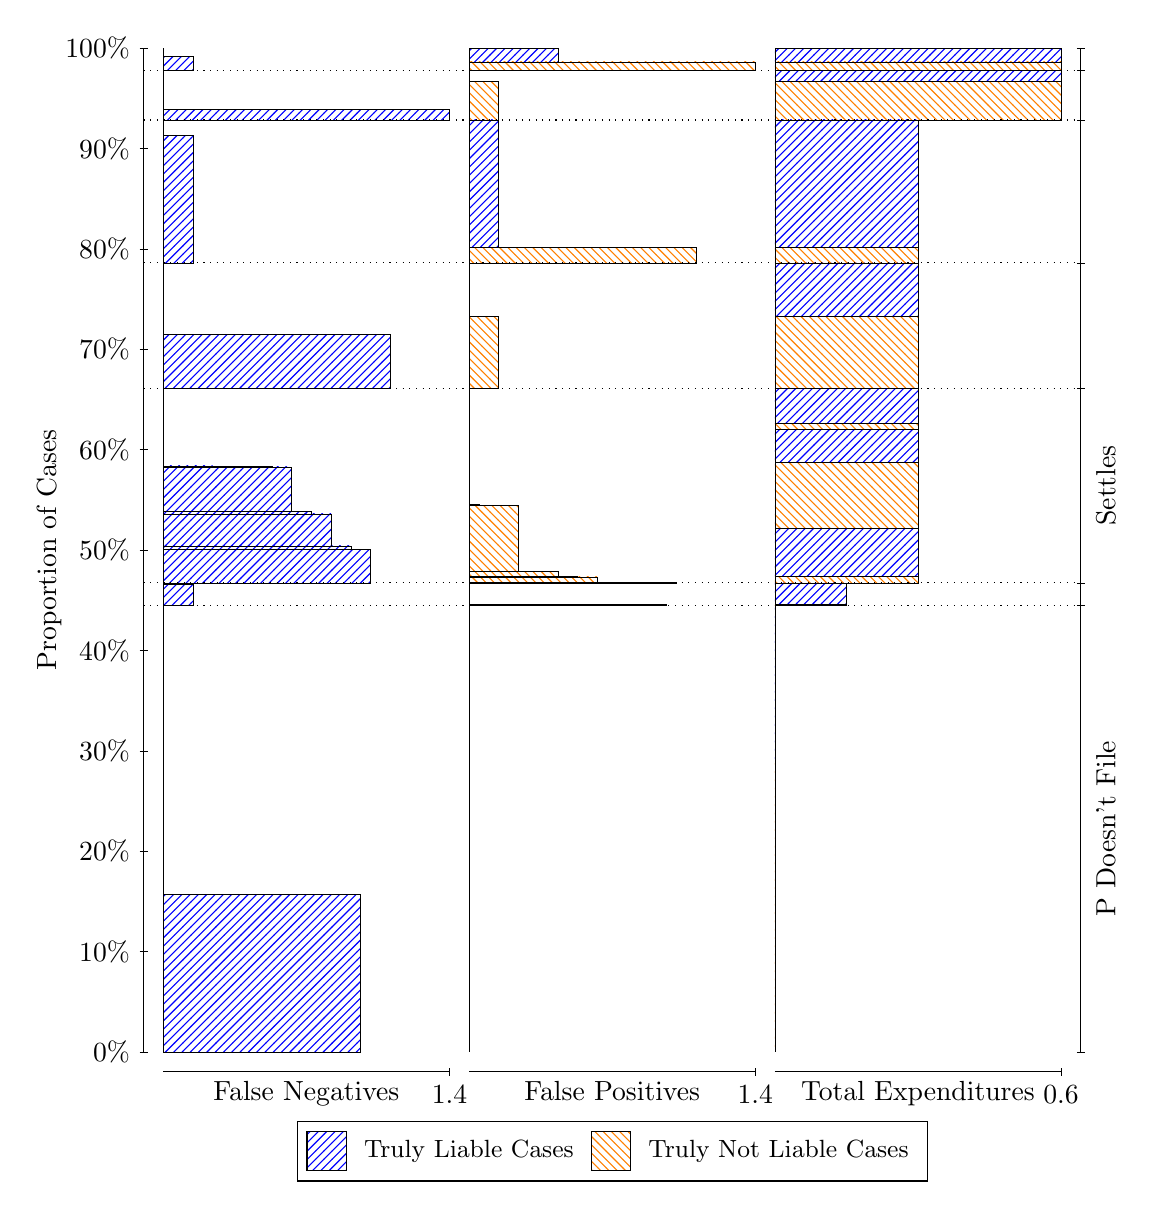
\begin{tikzpicture}
\draw[black, very thin] (1.5,1.75) -- (1.5,14.5);
\node[rotate=90, anchor=center] at (0.3, 8.125) {Proportion of Cases};
\draw[black, very thin] (1.45,1.75) -- (1.55,1.75);
\node[anchor=east] at (1.45, 1.75) {0\%};
\draw[black, very thin] (1.45,3.025) -- (1.55,3.025);
\node[anchor=east] at (1.45, 3.025) {10\%};
\draw[black, very thin] (1.45,4.3) -- (1.55,4.3);
\node[anchor=east] at (1.45, 4.3) {20\%};
\draw[black, very thin] (1.45,5.575) -- (1.55,5.575);
\node[anchor=east] at (1.45, 5.575) {30\%};
\draw[black, very thin] (1.45,6.85) -- (1.55,6.85);
\node[anchor=east] at (1.45, 6.85) {40\%};
\draw[black, very thin] (1.45,8.125) -- (1.55,8.125);
\node[anchor=east] at (1.45, 8.125) {50\%};
\draw[black, very thin] (1.45,9.4) -- (1.55,9.4);
\node[anchor=east] at (1.45, 9.4) {60\%};
\draw[black, very thin] (1.45,10.675) -- (1.55,10.675);
\node[anchor=east] at (1.45, 10.675) {70\%};
\draw[black, very thin] (1.45,11.95) -- (1.55,11.95);
\node[anchor=east] at (1.45, 11.95) {80\%};
\draw[black, very thin] (1.45,13.225) -- (1.55,13.225);
\node[anchor=east] at (1.45, 13.225) {90\%};
\draw[black, very thin] (1.45,14.5) -- (1.55,14.5);
\node[anchor=east] at (1.45, 14.5) {100\%};

\draw[black, very thin] (13.4,1.75) -- (13.4,14.5);
\draw[black, very thin] (13.35,1.75) -- (13.45,1.75);
\node[anchor=west] at (13.35, 1.75) {};
\draw[black, very thin] (13.35,7.4217) -- (13.45,7.4217);
\node[anchor=west] at (13.35, 7.4217) {};
\draw[black, very thin] (13.35,7.7085) -- (13.45,7.7085);
\node[anchor=west] at (13.35, 7.7085) {};
\draw[black, very thin] (13.35,10.18) -- (13.45,10.18);
\node[anchor=west] at (13.35, 10.18) {};
\draw[black, very thin] (13.35,11.772) -- (13.45,11.772);
\node[anchor=west] at (13.35, 11.772) {};
\draw[black, very thin] (13.35,13.586) -- (13.45,13.586);
\node[anchor=west] at (13.35, 13.586) {};
\draw[black, very thin] (13.35,14.218) -- (13.45,14.218);
\node[anchor=west] at (13.35, 14.218) {};
\draw[black, very thin] (13.35,14.5) -- (13.45,14.5);
\node[anchor=west] at (13.35, 14.5) {};

\draw[black, very thin, pattern color=blue, pattern=north east lines] (1.75,1.75) rectangle (4.2557,3.7529);
\draw[black, very thin, pattern color=orange, pattern=north west lines] (1.75,3.7529) rectangle (1.75,7.4217);
\draw[black, very thin, pattern color=blue, pattern=north east lines] (1.75,7.4217) rectangle (2.1259,7.6924);
\draw[black, very thin, pattern color=orange, pattern=north west lines] (1.75,7.6924) rectangle (1.75,7.7085);
\draw[black, very thin, pattern color=blue, pattern=north east lines] (1.75,7.7085) rectangle (4.381,8.1332);
\draw[black, very thin, pattern color=blue, pattern=north east lines] (1.75,8.1332) rectangle (4.1305,8.1771);
\draw[black, very thin, pattern color=blue, pattern=north east lines] (1.75,8.1771) rectangle (3.8799,8.5831);
\draw[black, very thin, pattern color=blue, pattern=north east lines] (1.75,8.5831) rectangle (3.6293,8.6172);
\draw[black, very thin, pattern color=blue, pattern=north east lines] (1.75,8.6172) rectangle (3.3787,9.1817);
\draw[black, very thin, pattern color=blue, pattern=north east lines] (1.75,9.1817) rectangle (3.1282,9.1834);
\draw[black, very thin, pattern color=blue, pattern=north east lines] (1.75,9.1834) rectangle (2.8776,9.1866);
\draw[black, very thin, pattern color=blue, pattern=north east lines] (1.75,9.1866) rectangle (2.627,9.1875);
\draw[black, very thin, pattern color=blue, pattern=north east lines] (1.75,9.1875) rectangle (2.3764,9.1923);
\draw[black, very thin, pattern color=orange, pattern=north west lines] (1.75,9.1923) rectangle (1.75,10.18);
\draw[black, very thin, pattern color=blue, pattern=north east lines] (1.75,10.18) rectangle (4.6316,10.861);
\draw[black, very thin, pattern color=orange, pattern=north west lines] (1.75,10.861) rectangle (1.75,11.772);
\draw[black, very thin, pattern color=blue, pattern=north east lines] (1.75,11.772) rectangle (2.1259,13.393);
\draw[black, very thin, pattern color=orange, pattern=north west lines] (1.75,13.393) rectangle (1.75,13.586);
\draw[black, very thin, pattern color=blue, pattern=north east lines] (1.75,13.586) rectangle (5.3833,13.723);
\draw[black, very thin, pattern color=orange, pattern=north west lines] (1.75,13.723) rectangle (1.75,14.218);
\draw[black, very thin, pattern color=blue, pattern=north east lines] (1.75,14.218) rectangle (2.1259,14.396);
\draw[black, very thin, pattern color=orange, pattern=north west lines] (1.75,14.396) rectangle (1.75,14.5);
\draw[black, very thin, pattern color=orange, pattern=north west lines] (5.6333,1.75) rectangle (5.6333,5.4188);
\draw[black, very thin, pattern color=blue, pattern=north east lines] (5.6333,5.4188) rectangle (5.6333,7.4217);
\draw[black, very thin, pattern color=orange, pattern=north west lines] (5.6333,7.4217) rectangle (8.1391,7.4379);
\draw[black, very thin, pattern color=blue, pattern=north east lines] (5.6333,7.4379) rectangle (5.6333,7.7085);
\draw[black, very thin, pattern color=orange, pattern=north west lines] (5.6333,7.7085) rectangle (8.2644,7.7088);
\draw[black, very thin, pattern color=orange, pattern=north west lines] (5.6333,7.7088) rectangle (8.0138,7.7089);
\draw[black, very thin, pattern color=orange, pattern=north west lines] (5.6333,7.7089) rectangle (7.7632,7.7091);
\draw[black, very thin, pattern color=orange, pattern=north west lines] (5.6333,7.7091) rectangle (7.5126,7.7092);
\draw[black, very thin, pattern color=orange, pattern=north west lines] (5.6333,7.7092) rectangle (7.2621,7.7837);
\draw[black, very thin, pattern color=orange, pattern=north west lines] (5.6333,7.7837) rectangle (7.0115,7.7885);
\draw[black, very thin, pattern color=orange, pattern=north west lines] (5.6333,7.7885) rectangle (7.0115,7.7886);
\draw[black, very thin, pattern color=orange, pattern=north west lines] (5.6333,7.7886) rectangle (6.7609,7.8506);
\draw[black, very thin, pattern color=orange, pattern=north west lines] (5.6333,7.8506) rectangle (6.5103,7.856);
\draw[black, very thin, pattern color=orange, pattern=north west lines] (5.6333,7.856) rectangle (6.2598,8.6959);
\draw[black, very thin, pattern color=blue, pattern=north east lines] (5.6333,8.6959) rectangle (5.7586,8.7007);
\draw[black, very thin, pattern color=blue, pattern=north east lines] (5.6333,8.7007) rectangle (5.6333,10.18);
\draw[black, very thin, pattern color=orange, pattern=north west lines] (5.6333,10.18) rectangle (6.0092,11.09);
\draw[black, very thin, pattern color=blue, pattern=north east lines] (5.6333,11.09) rectangle (5.6333,11.772);
\draw[black, very thin, pattern color=orange, pattern=north west lines] (5.6333,11.772) rectangle (8.5149,11.965);
\draw[black, very thin, pattern color=blue, pattern=north east lines] (5.6333,11.965) rectangle (6.0092,13.586);
\draw[black, very thin, pattern color=orange, pattern=north west lines] (5.6333,13.586) rectangle (6.0092,14.081);
\draw[black, very thin, pattern color=blue, pattern=north east lines] (5.6333,14.081) rectangle (5.6333,14.218);
\draw[black, very thin, pattern color=orange, pattern=north west lines] (5.6333,14.218) rectangle (9.2667,14.323);
\draw[black, very thin, pattern color=blue, pattern=north east lines] (5.6333,14.323) rectangle (6.7609,14.5);
\draw[black, very thin, pattern color=orange, pattern=north west lines] (9.5167,1.75) rectangle (9.5167,5.4188);
\draw[black, very thin, pattern color=blue, pattern=north east lines] (9.5167,5.4188) rectangle (9.5167,7.4217);
\draw[black, very thin, pattern color=orange, pattern=north west lines] (9.5167,7.4217) rectangle (10.425,7.4379);
\draw[black, very thin, pattern color=blue, pattern=north east lines] (9.5167,7.4379) rectangle (10.425,7.7085);
\draw[black, very thin, pattern color=orange, pattern=north west lines] (9.5167,7.7085) rectangle (11.333,7.7885);
\draw[black, very thin, pattern color=blue, pattern=north east lines] (9.5167,7.7885) rectangle (11.333,8.3967);
\draw[black, very thin, pattern color=orange, pattern=north west lines] (9.5167,8.3967) rectangle (11.333,9.2366);
\draw[black, very thin, pattern color=blue, pattern=north east lines] (9.5167,9.2366) rectangle (11.333,9.6613);
\draw[black, very thin, pattern color=orange, pattern=north west lines] (9.5167,9.6613) rectangle (11.333,9.7288);
\draw[black, very thin, pattern color=blue, pattern=north east lines] (9.5167,9.7288) rectangle (11.333,10.18);
\draw[black, very thin, pattern color=orange, pattern=north west lines] (9.5167,10.18) rectangle (11.333,11.09);
\draw[black, very thin, pattern color=blue, pattern=north east lines] (9.5167,11.09) rectangle (11.333,11.772);
\draw[black, very thin, pattern color=orange, pattern=north west lines] (9.5167,11.772) rectangle (11.333,11.965);
\draw[black, very thin, pattern color=blue, pattern=north east lines] (9.5167,11.965) rectangle (11.333,13.586);
\draw[black, very thin, pattern color=orange, pattern=north west lines] (9.5167,13.586) rectangle (13.15,14.081);
\draw[black, very thin, pattern color=blue, pattern=north east lines] (9.5167,14.081) rectangle (13.15,14.218);
\draw[black, very thin, pattern color=orange, pattern=north west lines] (9.5167,14.218) rectangle (13.15,14.323);
\draw[black, very thin, pattern color=blue, pattern=north east lines] (9.5167,14.323) rectangle (13.15,14.5);
\draw[black, dotted] (1.5,7.4217) -- (13.4,7.4217);
\draw[black, dotted] (1.5,7.7085) -- (13.4,7.7085);
\draw[black, dotted] (1.5,10.18) -- (13.4,10.18);
\draw[black, dotted] (1.5,11.772) -- (13.4,11.772);
\draw[black, dotted] (1.5,13.586) -- (13.4,13.586);
\draw[black, dotted] (1.5,14.218) -- (13.4,14.218);
\draw[black, very thin] (1.75,1.5) -- (5.3833,1.5);
\node[anchor=north] at (3.5667, 1.5) {False Negatives};
\draw[black, very thin] (5.3833,1.45) -- (5.3833,1.55);
\node[anchor=north] at (5.3833, 1.45) {1.4};

\draw[black, very thin] (5.6333,1.5) -- (9.2667,1.5);
\node[anchor=north] at (7.45, 1.5) {False Positives};
\draw[black, very thin] (9.2667,1.45) -- (9.2667,1.55);
\node[anchor=north] at (9.2667, 1.45) {1.4};

\draw[black, very thin] (9.5167,1.5) -- (13.15,1.5);
\node[anchor=north] at (11.333, 1.5) {Total Expenditures};
\draw[black, very thin] (13.15,1.45) -- (13.15,1.55);
\node[anchor=north] at (13.15, 1.45) {0.6};

\node[black, centered, rotate=90] at (13.72, 4.5858) {P Doesn't File};

\node[black, centered, rotate=90] at (13.72, 8.9441) {Settles};





\draw (7.449999999999999,1.5) node[draw=none] (baseCoordinate) {};
\begin{scope}[align=center]
        \matrix[scale=0.5, draw=black, below=0.5cm of baseCoordinate, nodes={draw}, column sep=0.1cm]{
            \node[rectangle, draw, minimum width=0.5cm, minimum height=0.5cm, pattern=north east lines, pattern color=blue] {}; &
            \node[draw=none, font=\small] (B) {Truly Liable Cases}; &
            \node[rectangle, draw, minimum width=0.5cm, minimum height=0.5cm, pattern=north west lines, pattern color=orange] {}; &
            \node[draw=none, font=\small] (B) {Truly Not Liable Cases}; \\
            };
\end{scope}

\end{tikzpicture}
\end{document}